\section{Hardware Components}

A design goal for the FEC upgrade was to obtain a higher light yield for PCAL compared to EC, but at a lower cost.  Since the early 1990s when EC was designed, lowered costs for the production of wavelength shifting (WLS) fibers combined with new techniques for the production of high light yield extruded scintillator, has enabled this cost savings.  Use of embedded WLS fibers bypasses the need for highly transparent scintillator (such as the long attenuation length BC-412 used in EC) and simplifies the readout which further improves the light yield.

Several studies were performed \cite{2007002,2007007,2009018} to select the optimal combination of light readout components (scintillator, WLS fiber and photomultiplier) needed to maximize the light yield.  Based on the results of measurements and the available price estimates, we concluded that the best choice for the PCAL components were: Fermilab (FNAL) extruded scintillator, the KURARAY Y11 1 mm diameter, multiclad WLS fiber, and the HAMAMATSU R6095 PMT, selected to have quantum efficiency $>$ 16$\%$ at 500 nm. It should be noted that the performance and price of extruded scintillators from Amcrys-Plast/Kharkov (Ukraine), WLS fibers G91A from BICRON and the HAMAMATSU PMT R1450 (selected to have $>$ 18$\%$ quantum efficiency at 500 nm) were not far from the best choice set and generally met the requirements for PCAL.    

\subsection{Scintillators}

The scintillator strips used in PCAL were manufactured at the FNAL-NICADD Extrusion Line Facilty.  The nominal dimensions were 500 mm x 45 mm x 10 mm. The polystryene base of the scintillators was Dow STYRON 663 W. The primary dopant was 2,5-diphenyloxazole (PPO, 1$\%$ by weight). The secondary dopant was 1,4-bis (5-phenyloxazol- 2-yl) benzene (POPOP, 0.03$\%$ by weight).  A reflective surface coating of polystryene with 12$\%$ TiO2 of 0.25 mm nominal thickness was co-extruded during the manufacturing process.  Each strip has two holes through the length of the strip which were also co-extruded. The holes are intended to allow easy insertion of two 1 mm diameter fibers.

Scintillators from FNAL were delivered to JLAB with two lengths: 420 cm (1450 strips used for U-views) and 450 cm (2710 strips used for V,W-views).   Cutting of the strips was performed at JLAB and at the College of William and Mary (WM). The average width for scintillators to be used in a given layer was measured before the scintillators were cut, and the final cut length of the strips needed to fit within the triangular area was chosen based on this average to avoid buildup of errors during stacking.  The largest deviation from the design width of 45 mm was less than 0.3 mm, compared to the specified  tolerance for this dimension of $\pm$~1 mm.

\subsection{Wave Shifting Fibers}
Charged particles traversing the scintillator strips excite an emission spectrum ranging between 370-450 nm. The photons are down-converted and transported to the photomultipliers via the WLS fibers. An initial design for the fiber readout proposed using three WLS green fibers embedded in straight grooves running the length of the scintillator surface, and the R$\&$D studies discussed above \cite{2007007} were based on prototypes of this configuration.  A later study \cite{2009018} showed that through-holes inside the scintillator would enhance the light yield, since the fiber would be fully enclosed. The question arose as to how the holes can be efficiently filled with epoxy for the large scintillator pieces avoiding air bubbles and pockets. Also it was important to characterize the light tranmission characteristics of the scintillator with and without epoxy.

Finally it was concluded \cite{2010012} that while a gluing procedure could be developed with good reproducibility, careful and time consuming attention was required for large scale production.  These same studies also showed that two WLS fibers per hole without glue gives approximately the same transmission characteristics as a single fiber with glue (Fig. \ref{fig:S4_4}.  It was also found that greater attenuation lengths were produced without gluing the fibers. The added expense of extra fiber was more than offset by a much faster and simplier assembly procedure together with a likely more uniform light collection efficiency. 

\begin{figure}[hbt]
\centering
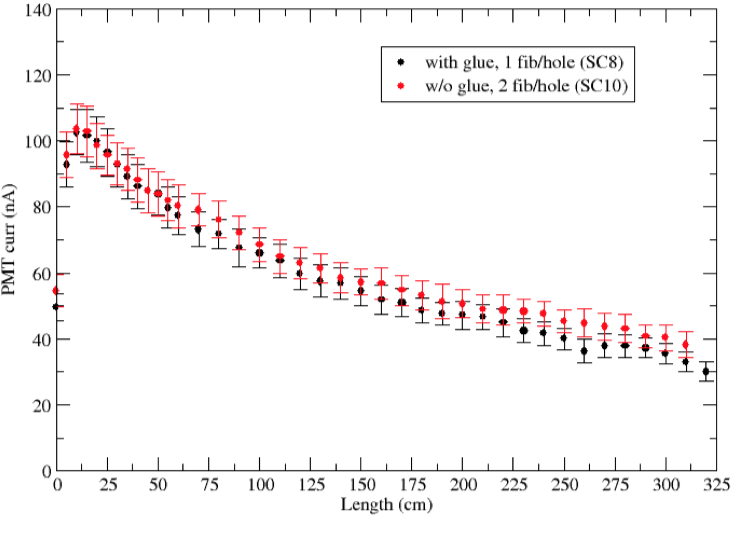
\includegraphics[width=0.85\columnwidth,keepaspectratio]{img/S4_4.png}
\caption{Relative light yield of various WLS readout fiber configurations.  Top and bottom plots compare different gluing procedures for fibers secured in holes filled with epoxy.}
\label{fig:S4_4}
\end{figure}

\subsection{Photomultiplier tubes}

\subsection{Lead}

Between two scintillator layers, there is one lead layer. For each PCAL module, there are a total of 14 lead layers. Each layer consists of two right-angle triangle shaped sheets, where the hypotenuse of each triangle is parallel to the V or W sidewall. Thickness uniformity of each layer was checked using a CHECK·LINE TI-25DL ultrasonic thickness gauge with 72 sample points measured per layer (36 for each half-layer).  Distributions of these sample points from all 14 layers in each module is shown in Fig. \ref{fig:S4_5}.

\begin{figure}[hbt]
\centering
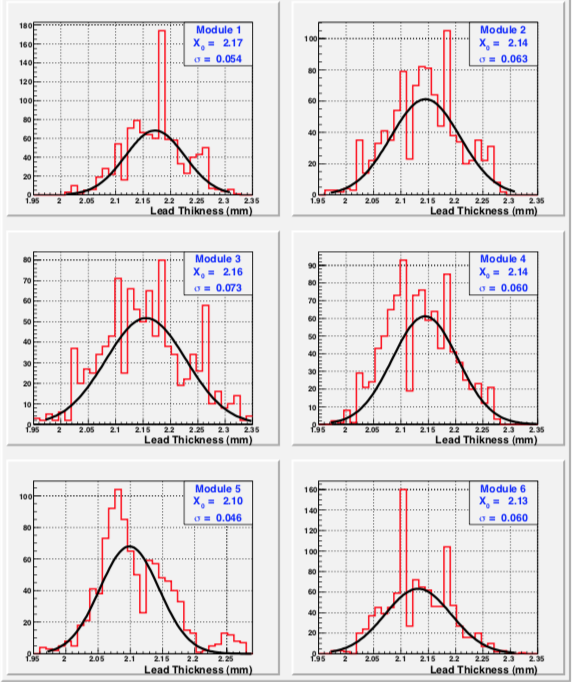
\includegraphics[width=0.95\columnwidth,keepaspectratio]{img/S4_5.png}
\caption{The distribution of measured thicknesses of the lead sheets for each PCAL module.}
\label{fig:S4_5}
\end{figure}


\section{Construction and Installation}
Construction steps include cleaning and assembly of the PCAL box, followed by stacking of the scintillator strips and lead sheets, routing of WLS fibers and spot gluing at both ends, milling and polishing of WLS fibers at the PMT readout housing and ending with final shimming and installation of the last composite window. Prior to installation, light transmission properties of the scintillators and WLS fibers were obtained in a test setup. 
\begin{figure}[hbt]
\centering
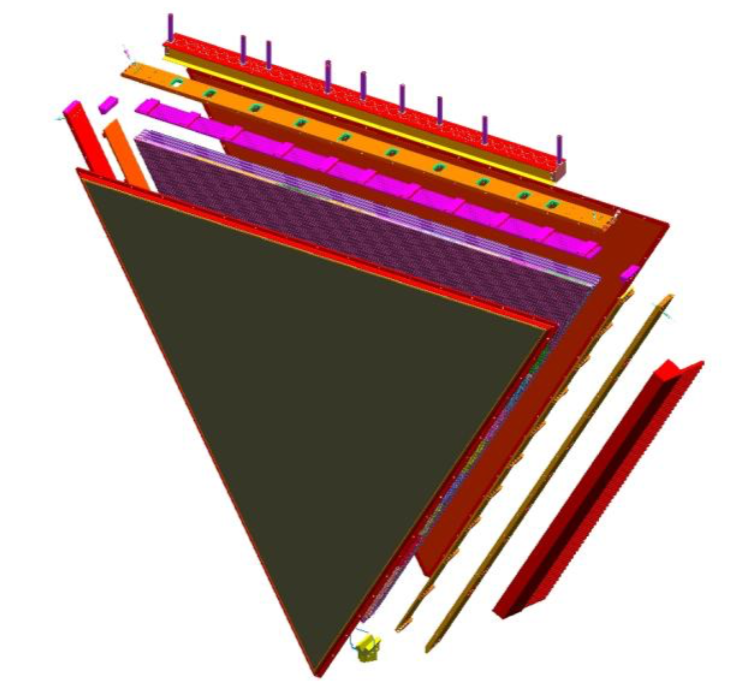
\includegraphics[width=0.95\columnwidth,keepaspectratio]{img/S5_1.png}
\caption{Three dimensional CAD model of the PCAL box showing the front/rear composite windows, sidewall supports and lead/scintillator sandwich.}
\label{fig:S5_1}
\end{figure}

\subsection{Mechanical support}

\subsection{Cutting of scintillator strips}
Scintillator strips for PCAL were received from FNAL in two lengths, 420 cm (1450 strips) and 450 cm (2710 strips). The shorter strips were used for the U view and the longer strips for the V- and W-views. To fit within the isosceles triangle shape, U strips have the same $27.1^\circ$ angle cut at both ends, while one end of the V- and W-strips has a $27.1^\circ$ cut, and the second end at the base of the triangle has a $35.8^\circ$ angle cut.

\subsection{Scintillator and WLS fiber testing}
In order to achieve a uniform response over the area covered by the PCAL, the transmission properties of the scintillator bars needs to be characterized. To minimize the data acquisition time, we will measure the PMT anode average current produced as a result of the irradiation of a radioactive source (90Sr beta source) at different positions of the scintillator bar. For the first sector, we will do the measurements for all of the longest (>200 cm) scintillator bars. The apparatus consists of a PMT to measure the response of the scintillator-fiber system and a radioactive source, which is mounted on a holder that is positioned on the top of a system that can be moved automatically along the length of the scintillator strip (see Figure 7 below).

\subsection{Lead-scintillator stacking}
Various elements of the PCAL box were cleaned with isopropanol to remove grease and debris from machining.  The bottom window was placed on a support table and side walls and retainers installed. Prior to scintillator stacking a 50$\mu$ Teflon sheet was laid down, followed by placement of the first U layer of 84 scintillator strips, beginning with the longest strip.
\subsection{WLS fiber routing}

\subsection{PMT installation}
\subsection{Installation in Hall B}









